\section{Anhang}
\label{sec:attachment}


\subsection{Beispiel Aufgabe}
\label{exercise}

In diesem Abschnitt wird der Umgang und die Bedienung der Erweiterung anhand einer Beispielaufgabe dargestellt. Die Aufgabe wurde aus dem Buch ``Tabellenkalkulationssysteme Datenbanken''~\cite{hubwieser_inf_2} von Seite 110 gewählt und ist eine Aufgabe die für die Zielgruppe (Kapitel: ~\ref{subsubsec03:zielgruppe}) der Erweiterung angemessen ist.

\begin{description}
\item[Aufgabenstellung] \hfill\\
In dieser Aufgabe soll ein ER-Diagramm in ein relationales Datenbankmodell überführt werden. Das ER-Diagramm ist in der Abbildung~\ref{pic:exercise} zu sehen. \textit{In der original Aufgabe besaßen die Entitytypen keine Attribute, diese wurden zur besseren Präsentation der Erweiterung hinzugefügt~\ref{pic:exercise_extended}.}

\begin{figure}[h]
  \begin{subfigure}[b]{0.45\textwidth}
    \includegraphics[width=\textwidth]{images/aufg_norm.pdf}
    \caption{Originale Aufgabenstellung}
    \label{pic:exercise}
  \end{subfigure}\hfill
  \begin{subfigure}[b]{0.45\textwidth}
    \includegraphics[width=\textwidth]{images/aufg_extra.pdf}
    \caption{Erweiterte Aufgabenstellung}
    \label{pic:exercise_extended}
  \end{subfigure}
\end{figure}

\item[Projekt öffnen] \hfill\\
Im ersten Schritt muss das passende Projekt geöffnet werden. Dafür wird in der Projektauswahl das Projekt ``Klett - Informatik 2'' durch den ``Bearbeitungs'' Button gewählt.

\begin{figure}[ht]
    \frame{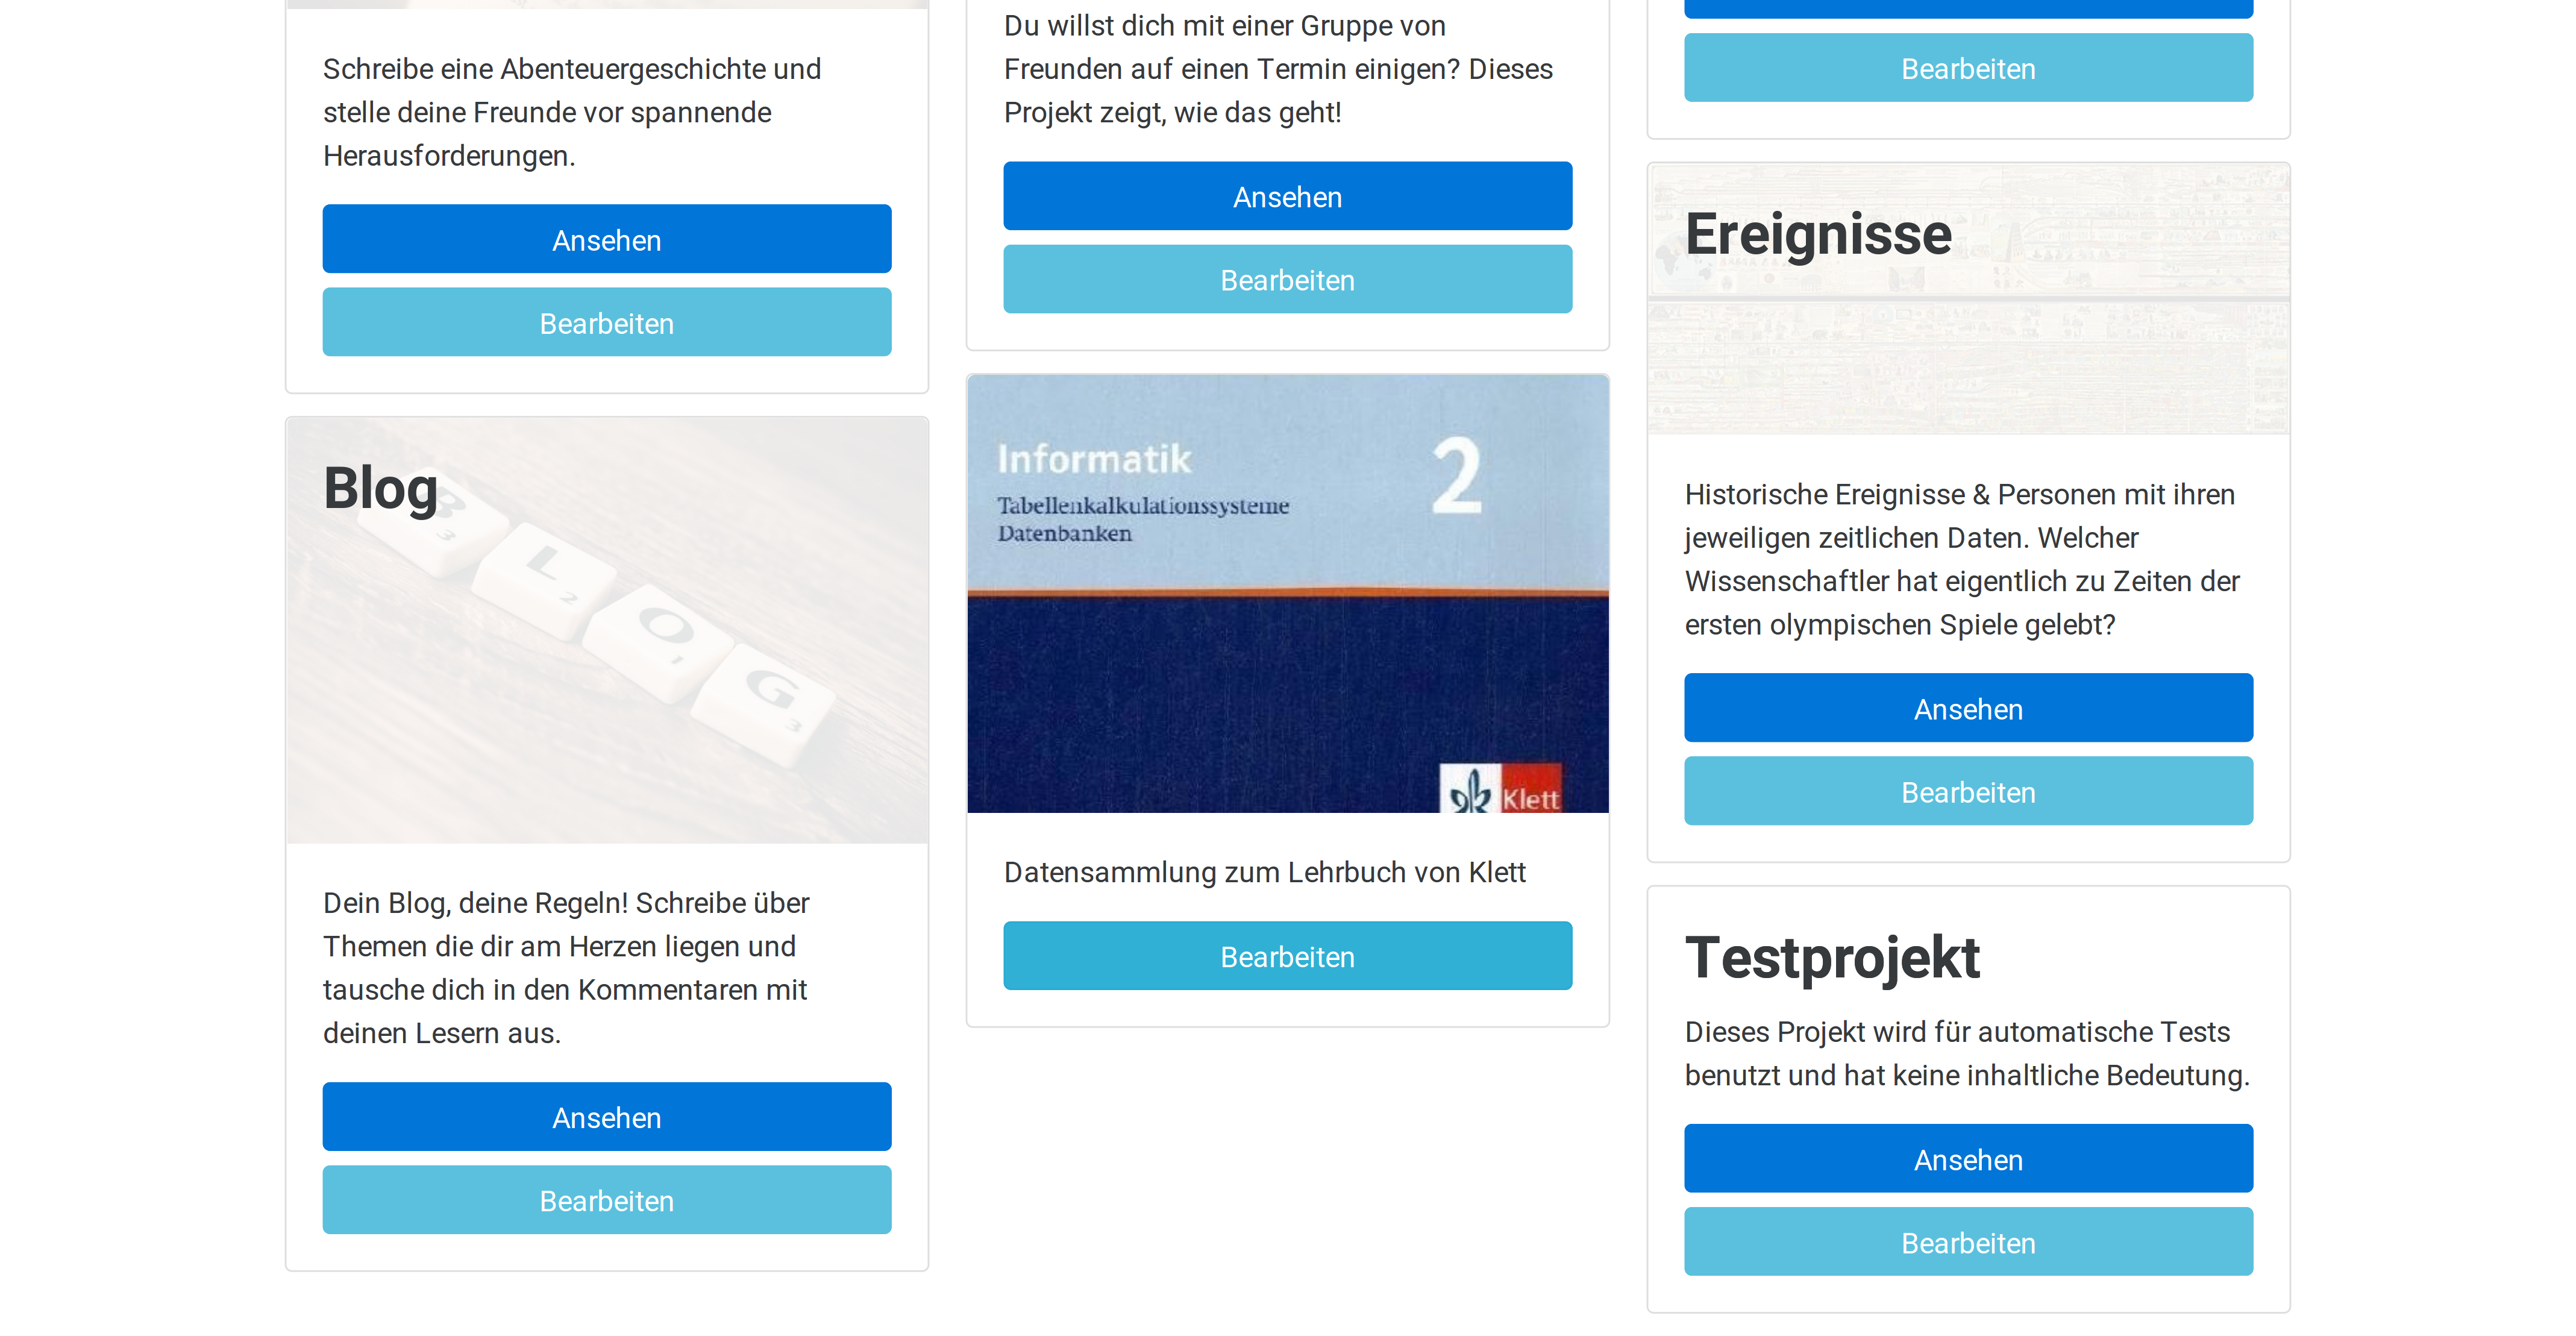
\includegraphics[width=\textwidth]{images/att-select-project.png}}
        \centering
        \caption{Projekt Auswahl}
        \label{pic:project_select}
\end{figure}


\item[Schema Ansicht] \hfill\\
Um Tabellen anlegen zu können, muss in die Schemaansicht gewechselt werden. Das Schema ist am Anfang leer, somit ist die einzige verfügbare Funktion eine neue Tabelle zu erstellen. Diese Funktion ist am oberen Rand durch den Button ``Neue Tabelle'' (Abbildung: ~\ref{pic:btn_new_table}) erreichbar.

\begin{figure}[ht]
    \frame{
\includegraphics[width=0.5\textwidth]{images/att-newtablebtn.png}}
        \centering
        \caption{Button zum Erstellen neuer Tabellen}
        \label{pic:btn_new_table}
\end{figure}

\item[Tabellen erstellen] \hfill\\
Durch den Button wird der Editor geöffnet. Im Editor können durch die einzelnen Bedienelemente eine Tabelle erstellt werden. Als ersten wird die Schüler Tabelle erstellt. \\

Im oberen Input Feld kann der Name der Tabelle, hier ``Schueler'', eingetragen werden. Nachdem die Tabelle einen Namen besitzt, müssen die einzelnen Spalten erzeugt werden. \\
Mit dem Klick auf das ``+''-Symbol kann eine neue Spalte hinzugefügt werden. Jeder Schüler soll einen Namen erhalten. 
In der neuen Spalte wird, wie bei der Tabelle, in dem ersten Input Feld der Name der Spalte ``Vorname'' eingetragen. Der Vorname ist kein Primärschlüssel somit wird die Checkbox nicht ausgewählt. Der Typ der Spalte wird in dem Dropdown-Menu ausgewählt. Zur Verfügung stehen:
\begin{itemize}
    \item TEXT
    \item INTEGER
    \item FLOAT
    \item BOOLEAN
    \item URL
\end{itemize} 
Für den Vornamen wird der Typ ``TEXT'' gewählt.
Jeder Schüler hat einen Namen, somit kann in die Checkbox ``NOT NULL'' ausgewählt. Einen Standartwert wird hier nicht vergeben. \\
Nach dem gleichen Schema wird nun eine Spalte für den ``Nachname'' erzeugt.
Um die einzelnen Schüler zu identifizieren wird noch eine zusätzliche Spalte benötigt.
Die zusätzliche künstliche Spalte erhält den Namen ``ID''. Diese Spalte soll als Primärschlüssel dienen, somit wird die Checkbox ausgewählt. Dabei wird ``NOT NULL'' automatisch gesetzt. Die ID Spalte ist vom Typ ``INTEGER''. Ein Standartwert wird nicht benötigt. \\
Zur besseren Gestaltung soll der Primärschlüssel die erste Spalte sein. Um die Spalte an diese Position zu verschieben, wählen wir im ersten Dropdown-Menu in der ``Switch'' Einstellung, die Spalte ``ID''. In dem zweiten Dropdown-Menu wird die Position gewählt. Die Einstellung wird mit dem nebenstehenden Button bestätigt.

Die fertige Tabelle sollte folgendermaßen aussehen: (Abbildung: ~\ref{pic:table-schueler})

\begin{figure}[ht]
    \frame{\includegraphics[width=\textwidth]{images/att-table-schueler.png}}
        \centering
        \caption{Fertige Schueler Tabelle}
        \label{pic:table-schueler}
\end{figure}

Die Tabelle ``Fach'' wird nach dem gleichen Muster erstellt. (Abbildung: ~\ref{pic:table-fach})

\begin{figure}[ht]
    \frame{\includegraphics[width=\textwidth]{images/att-table-fach.png}}
        \centering
        \caption{Fertige Fach Tabelle}
        \label{pic:table-fach}
\end{figure}

\item[Beheben von Fehlern] \hfill\\
Sollte während der Bearbeitung ein Fehler passieren, kann der ``Undo'' Button auf der oberen Seite verwendet werden. Zusätzlich wird nach jeder Änderung ein Eintrag im Stack erstellt. Mit einem Mausklick auf einen Stackeintrag wird die Tabelle zu diesem Zustand verändern.

\item[Vereinigungstabelle erstellen] \hfill\\
Da die Relation zwischen den Tabellen eine N-zu-M-Relation ist, muss zusätzlich eine Vereinigungstabelle erstellt werden.
Zuerst wird eine neue Tabelle namens ``macht\_\-Abi'' erstellt, die nur die Spalte ``Note'' vom Typ ``FLOAT'' besitzt. Für diese Spalte wird der Standartwert ``0.0'' eingetragen. \\
Nach dem Speichern der Tabelle, wird in der Schemaansicht das Schema dargestellt (Abbildung: ~\ref{pic:no-rel}). Es ist zu sehen, dass die Tabellen keine Relation haben.


\begin{figure}[h]
  \begin{subfigure}[b]{0.45\textwidth}
    \includegraphics[width=\textwidth]{images/att-no-rel.png}
    \caption{Schema ohne Relationen}
    \label{pic:no-rel}
  \end{subfigure}\hfill
  \begin{subfigure}[b]{0.45\textwidth}
    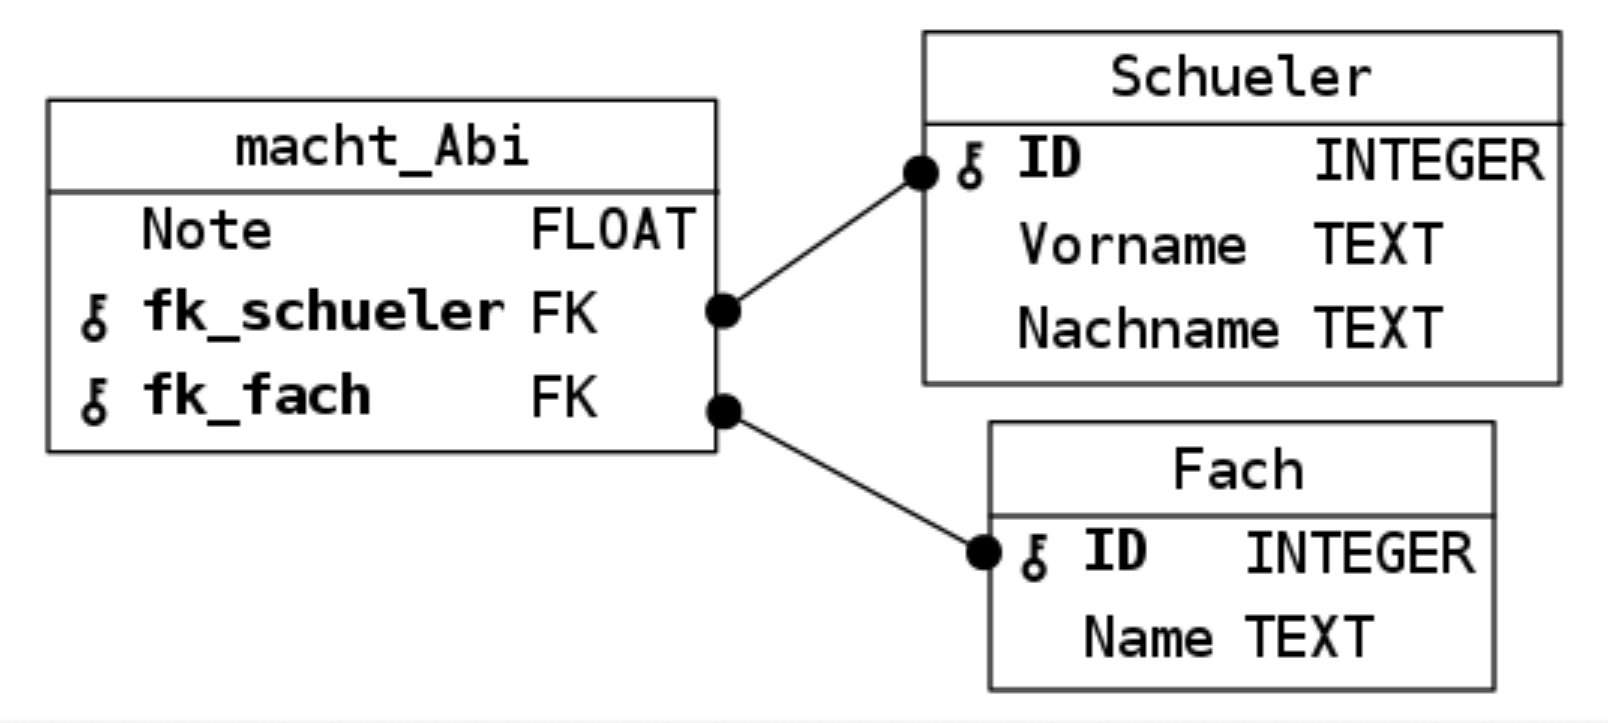
\includegraphics[width=\textwidth]{images/att-with-rel.png}
    \caption{Schema mit Relationen}
    \label{pic:with-rel}
  \end{subfigure}
\end{figure}


\item[Tabellen bearbeiten] \hfill\\
Um Relationen zwischen den Tabellen zu erstellen, muss die Tabelle ``macht\_\-Abi'' bearbeitet werden. Es wird auf das bearbeitungs Symbol neben der Tabelle gedrückt. Es werden zwei Spalten erstellt: ``fk\_\-schueler'' und ``fk\_\-fach'', die beide vom Typ ``INTEGER'' sind. \\
Die Spalten sollen Foreign Keys auf die beiden Tabellen haben. Im ersten Dropdown-Menu in der ``Add FK'' Auswahl, wird die Spalte ``fk\_\-schueler'' ausgewählt. In dem darauf erscheinten Dropdown-Menu wird die Tabelle gewählt auf den der Foreign Key zeigen soll. In diesem Fall ``Schueler''. In dem letzten Dropdown-Menu wird noch die genaue Spalte (``ID'') der Tabelle gewählt, auf den der Foreign Key verweisen soll. Nachdem alles ausgewählt wurde wird die Einstellung mit dem Button bestätigt. \\
Die Schritte werden für den Foreign Key zur ``Fach'' Tabelle erstellt.
Die erstellten Foreign Keys werden dabei unter dem Typen der Spalte dargestellt. Wenn die Tabelle folgendermaßen (Abbildung: ~\ref{pic:editor-fk}) aussieht, kann diese gespeichert werden. 

\begin{figure}[ht]
    \frame{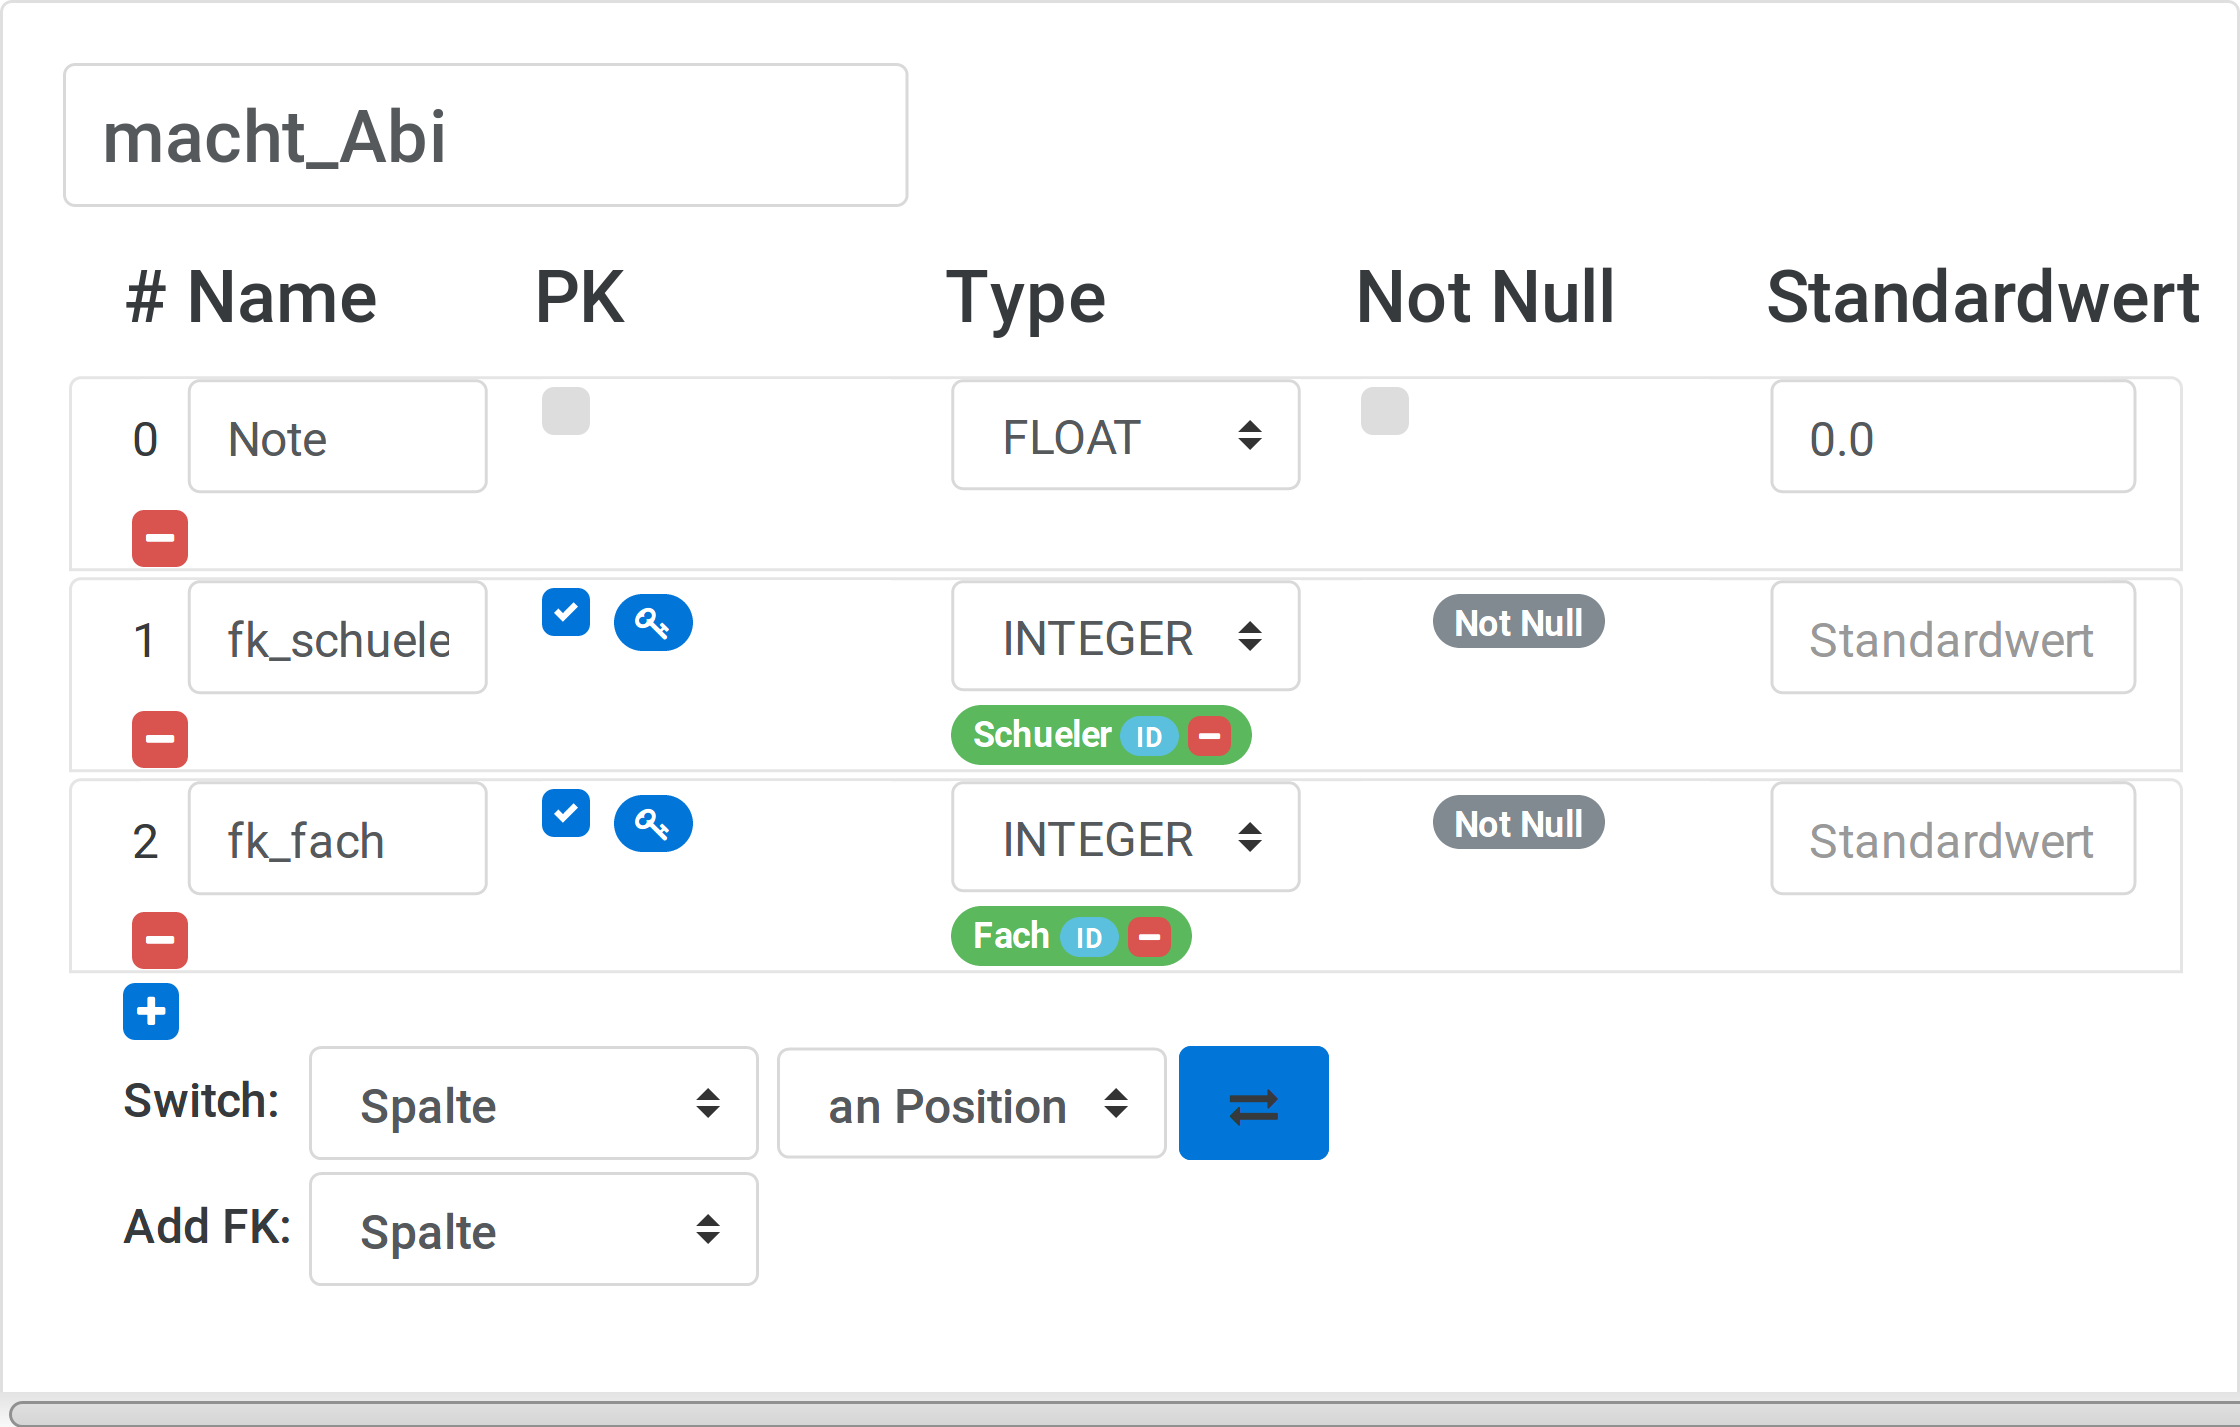
\includegraphics[width=\textwidth]{images/att-editor-fk.png}}
        \centering
        \caption{Tabelle mach\_Abi mit Foreign Keys}
        \label{pic:editor-fk}
\end{figure}

Das angezeigte Schema ist (Abbildung: ~\ref{pic:with-rel}) wie es zu erwarten ist.

\item[Tabellen Datten befüllen] \hfill\\
Nachdem das Schema erstellt wurde, können mit der bereits eingebauten Funktion Datensätze in die Tabelle eingeführt werden. (Abbildung: ~\ref{pic:insert-stat}) \textit{Für genauere Informationen dazu siehe die Master-Thesis von Marcus Riemer.}~\footnote{\url{https://marcusriemer.de/static/marcus-riemer-thesis-blattwerkzeug.pdf}}

\begin{figure}[ht]
    \frame{\includegraphics[width=\textwidth]{images/att-insert-stat.png}}
        \centering
        \caption{Insert Statement erstellen}
        \label{pic:insert-stat}
\end{figure}

\item[Tabelleninhalte ansehen] \hfill\\
Zum Schluss können, indem der Name der Tabelle geklickt wird, die eingetragenen Daten angezeigt werden.

\begin{figure}[ht]
    \frame{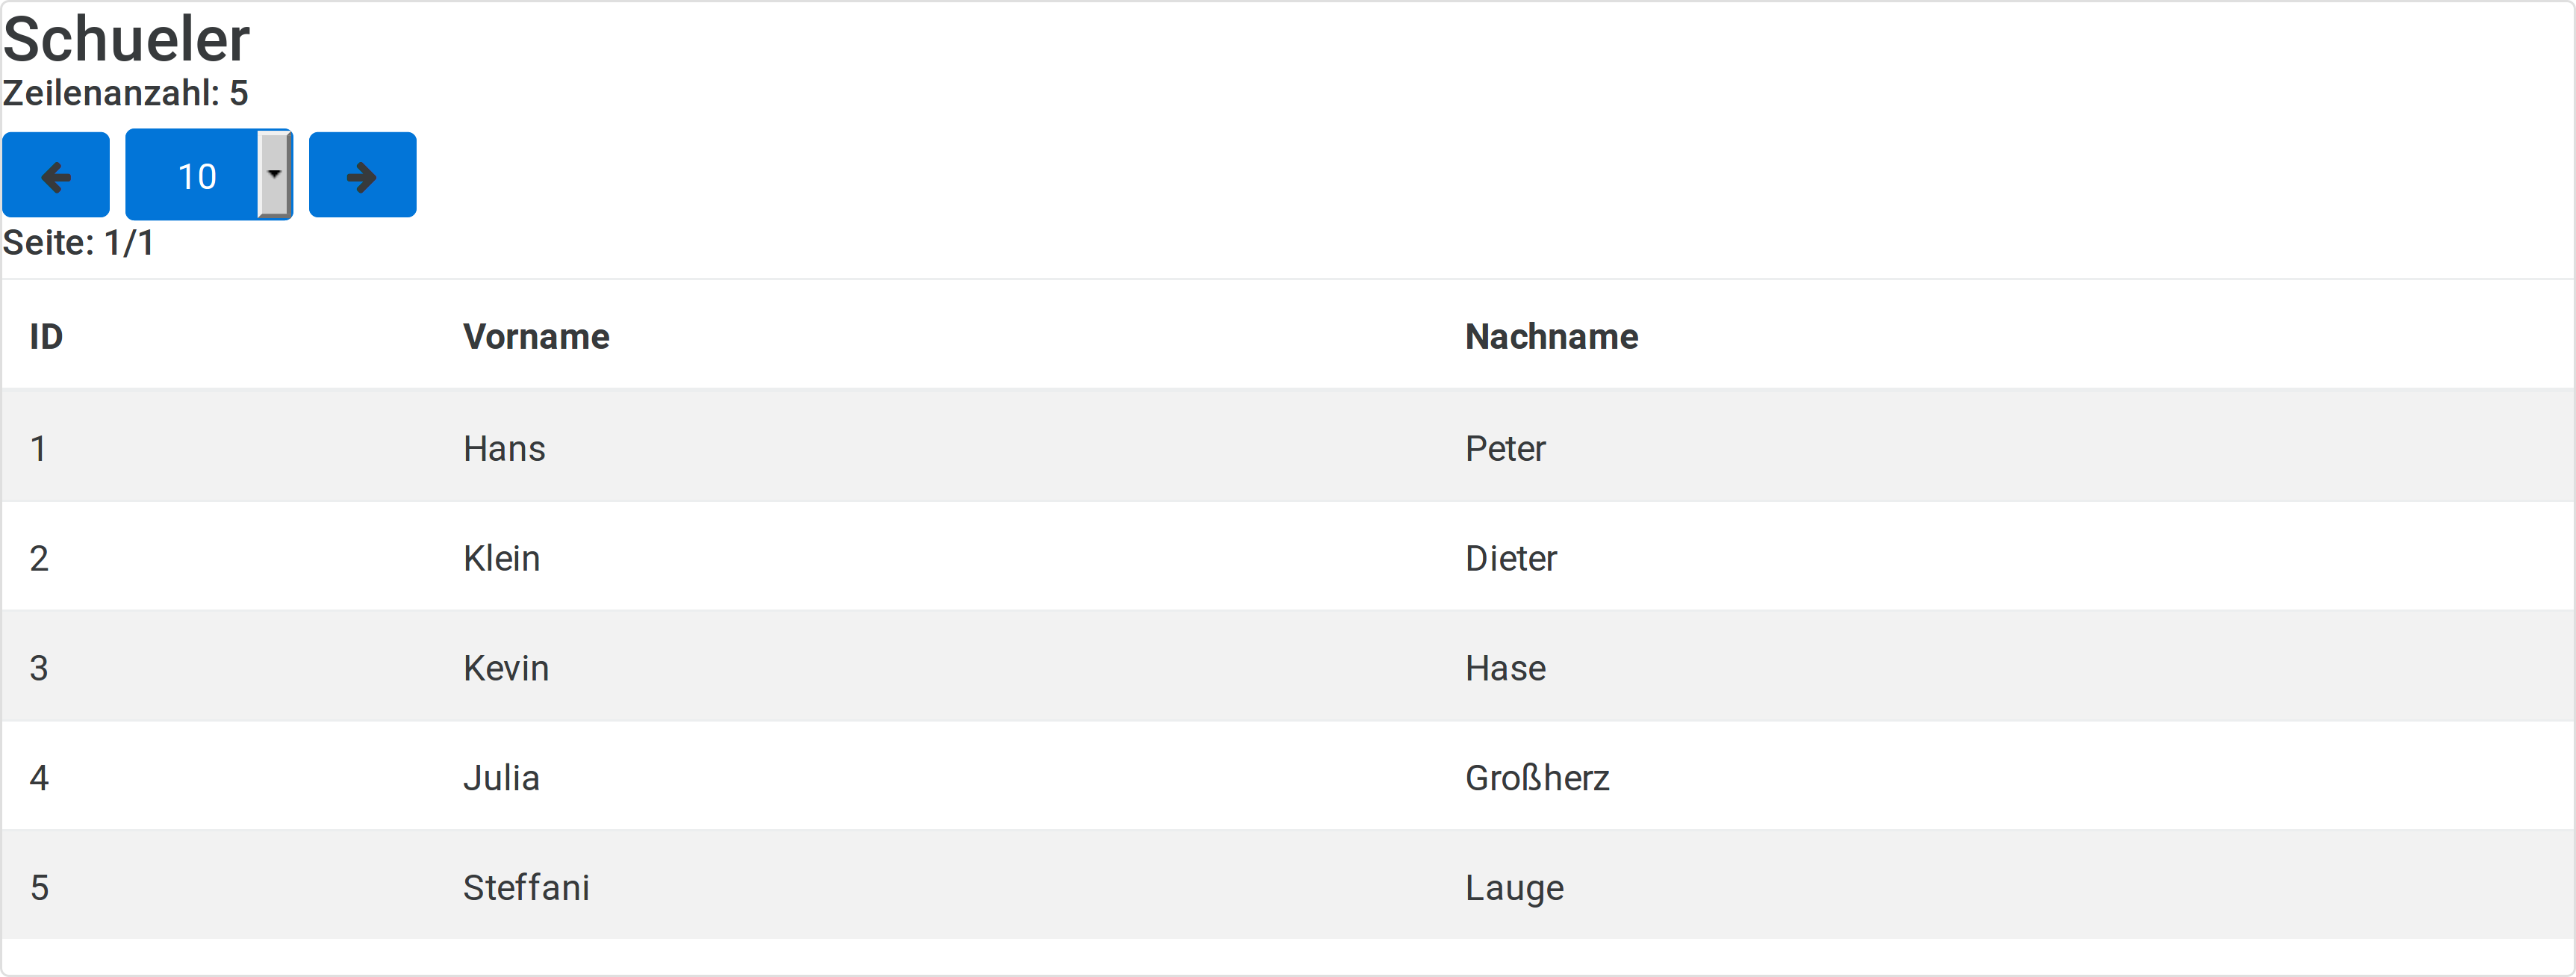
\includegraphics[width=\textwidth]{images/att-table-details.png}}
        \centering
        \caption{Tabelleninhalte der Schueler Tabelle}
        \label{pic:table-details}
\end{figure}

\end{description}

